\documentclass[a4paper,twoside]{article}

\usepackage{epsfig}
\usepackage{subfigure}
\usepackage{calc}
\usepackage{amssymb}
\usepackage{amstext}
\usepackage{amsmath}
\usepackage{multicol}
\usepackage{pslatex}
\usepackage{apalike}
\usepackage{fancyhdr}
\usepackage{scitepress}
\usepackage[small]{caption}
\usepackage{graphicx}
\usepackage{float}


\begin{document}
\onecolumn \maketitle \normalsize \vfill

\section{\uppercase{Introduction}}
\label{sec:introduction}
\noindent Large scale computer infrastructures such as grids and clouds are increasingly being used. The complexity of the network increases due to the a growing number of hardware and software components. The fact that these components can be owned by various organizations puts even more challenges on the level of service management. For the user most administrative issues are shielded behind the provider of the infrastructure. However, when confronted with failures or in case of unexpected performance, it appears to be very difficult to get a grip on the cause of the problem. In such cases a lot of communication between the user and one or more system administrators is needed, which is often perceived as a tedious or time consuming process. Furthermore, there is often a difference in the terminology used by a user and a system administrator. Translations between various concepts and scenarios have to be made which often leads to even more communication or worse: misunderstandings.
\\
In their task of operational grid-management administrators make comparisons, relate local events and communicate their findings with each other in their attempt to find possible causes of malfunctioning or under performance of the infrastructure. There is a strong need for automated verification methods that will increase the robustness and fault-tolerance of the infrastructure. These methods can be based on statistics extracted from the operational infrastructure and the correlation of data sets. The growth of these environments in terms of size and usage requires supporting systems to be of a sophisticated level. Autonomous, distributed and semantic techniques can overcome problems related to the dynamic multi domain nature of the environment.\\
As an example of such an approach and to investigate its viability we started a Project called DUST at the Academic Medical Center (AMC). With this project we aim to design, implement and deploy intelligent agents to assist experts and non-expert users to monitor the execution of workflows with MOTEUR on the Dutch Grid.

\section{\uppercase{The DUST project} }
\label{sec:dust}
\noindent
In this chapter we will present to you the details about the DUST project.

\subsection{Introduction}
\noindent
At the AMC various researchers run applications on the Dutch Grid. The applications are implemented as workflows defined in an XML dialect (SCUFL), and submitted to a MOTEUR server using a client called VBrowser. This setup should hide away the complexity of the underlying grid environment. To some extend this is successful, but in the case of failures specialists in the various domains have to collaborate in order to find the cause and solve the issue. A researcher is, apart from his core task to perform research, also involved in the development, monitoring and troubleshooting of the workflows.

\begin{figure}[H]
  \vspace{-0.2cm}
  \centering
  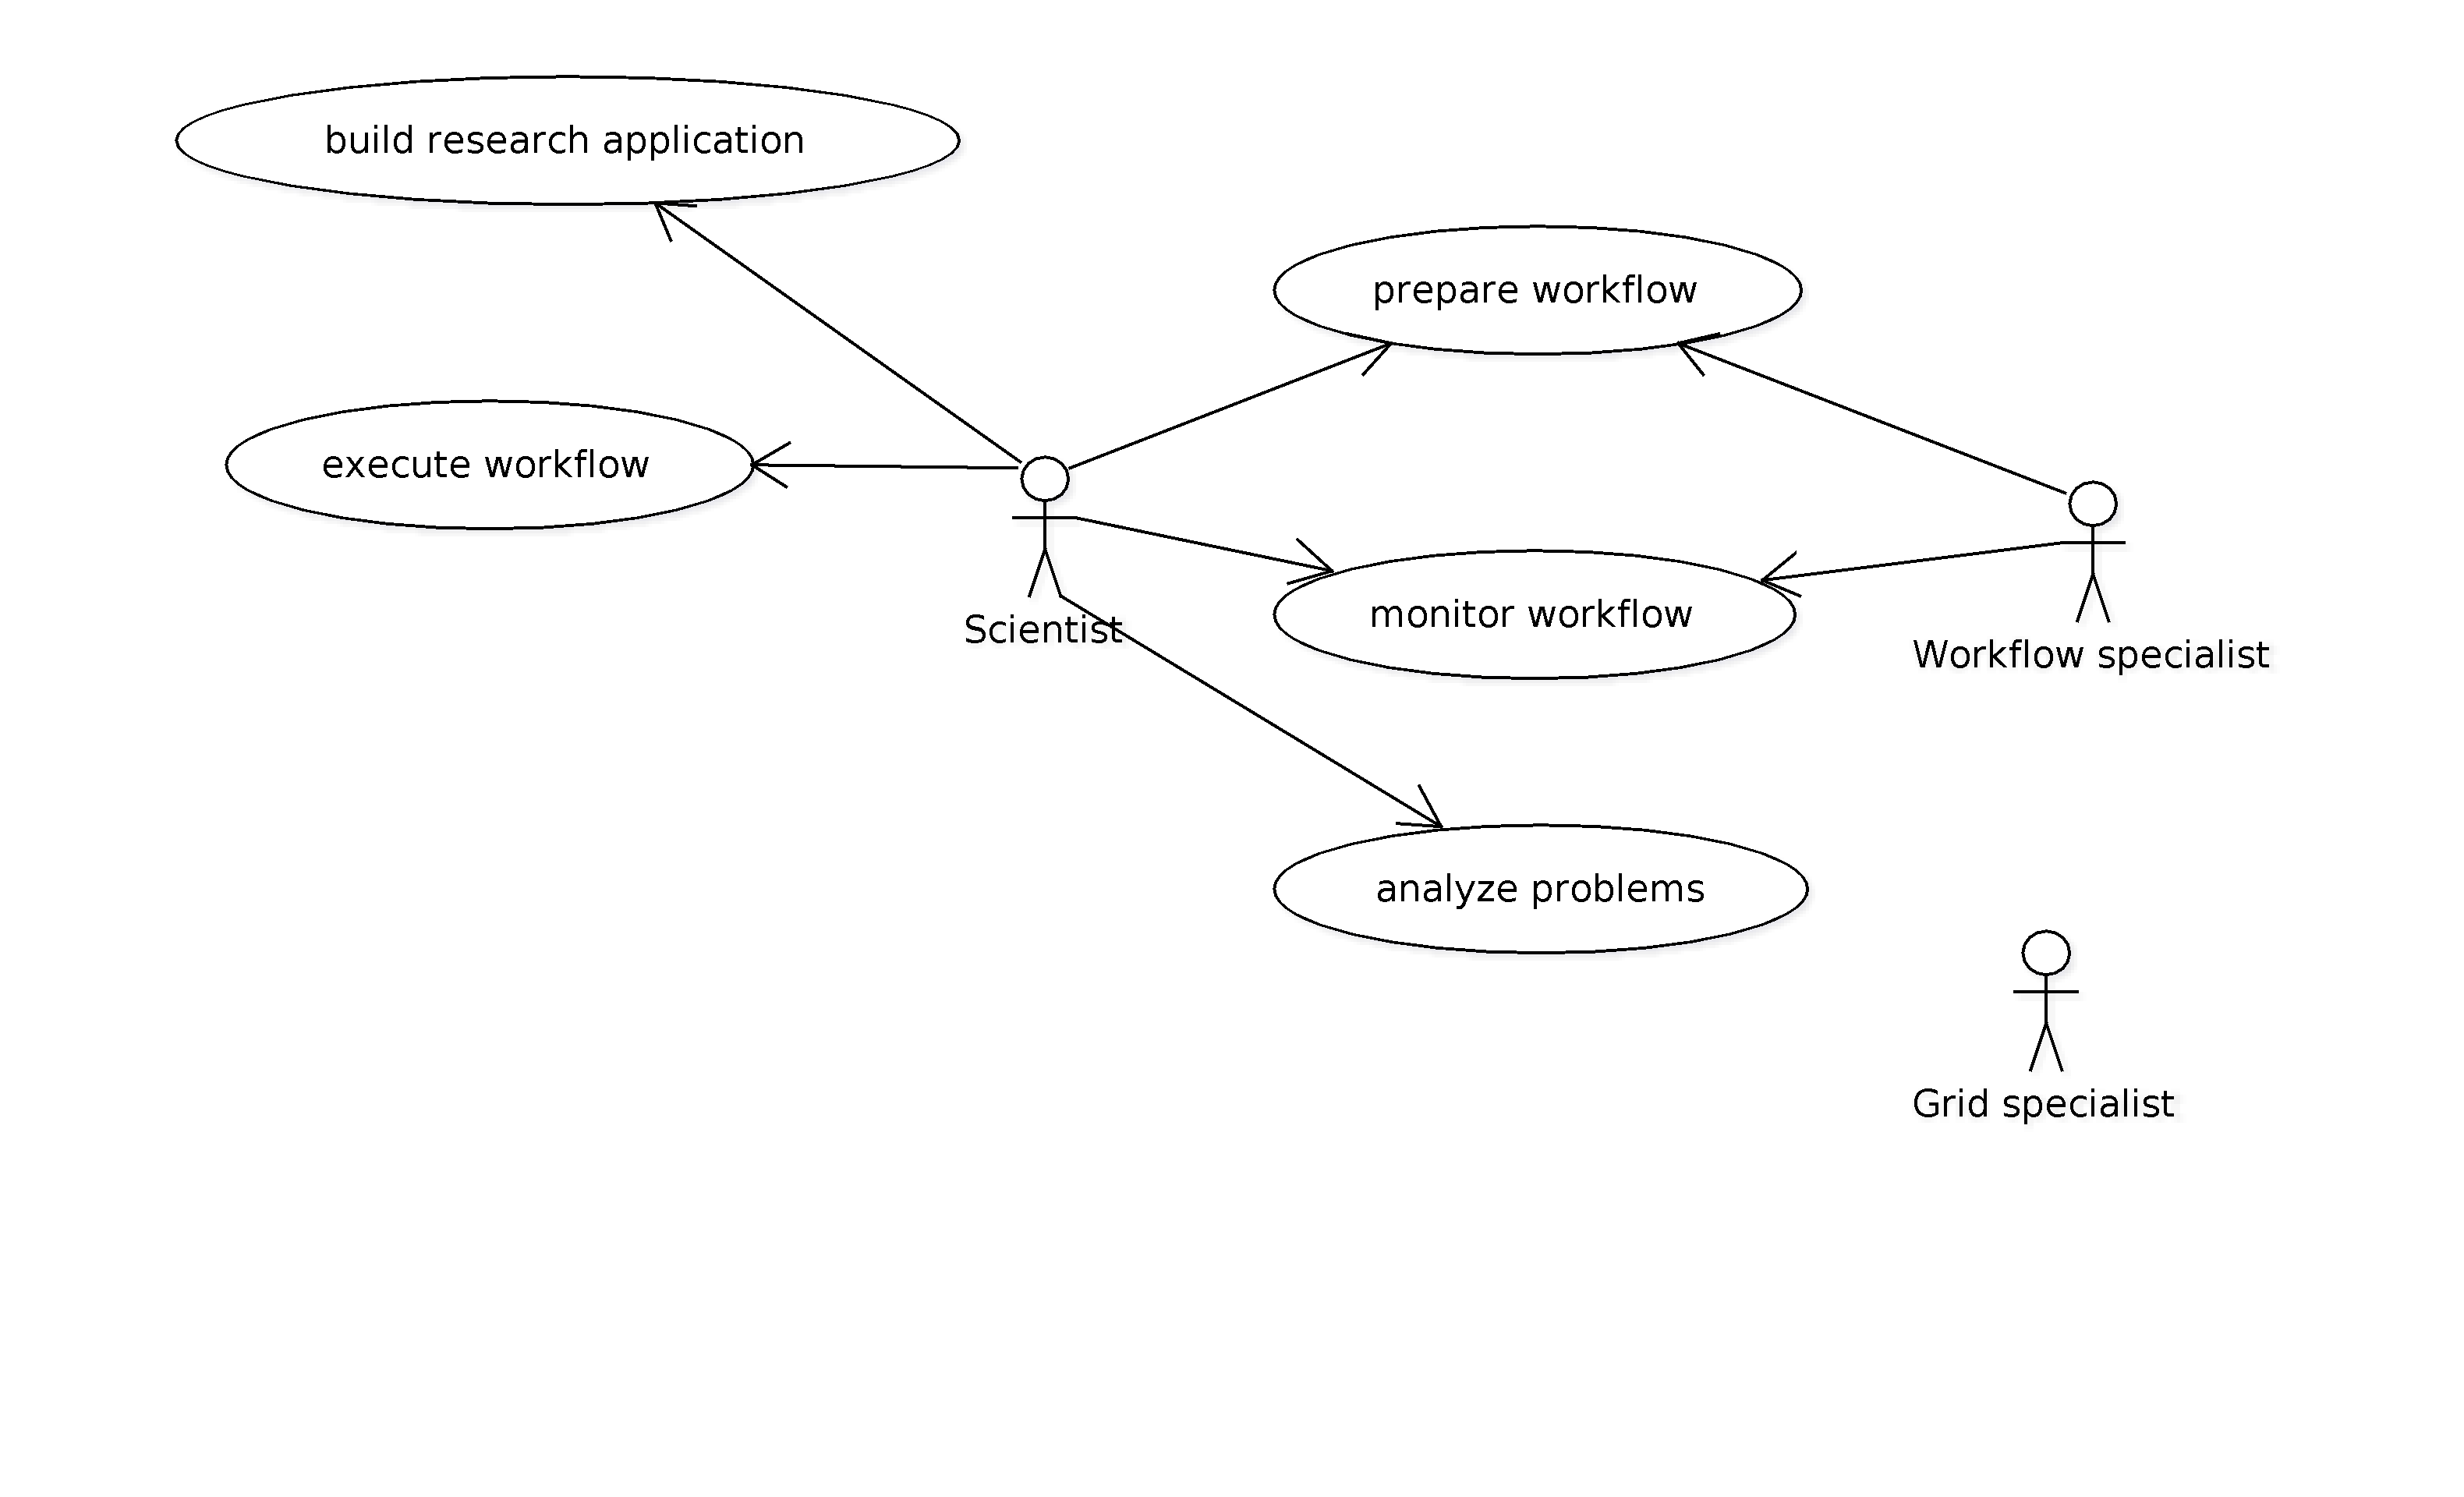
\includegraphics[width=7cm,height=4.6cm]{currentusecasegridresearchamc.png} 
  \caption{Usecase diagram showing people and tasks involved in grid research. }
  \label{fig:currentusecase}
  \vspace{-0.5cm}
\end{figure}

In order to run an experiment on the grid various applications in different domains are involved.

\begin{figure}[H]
  \vspace{-0.2cm}
  \centering
  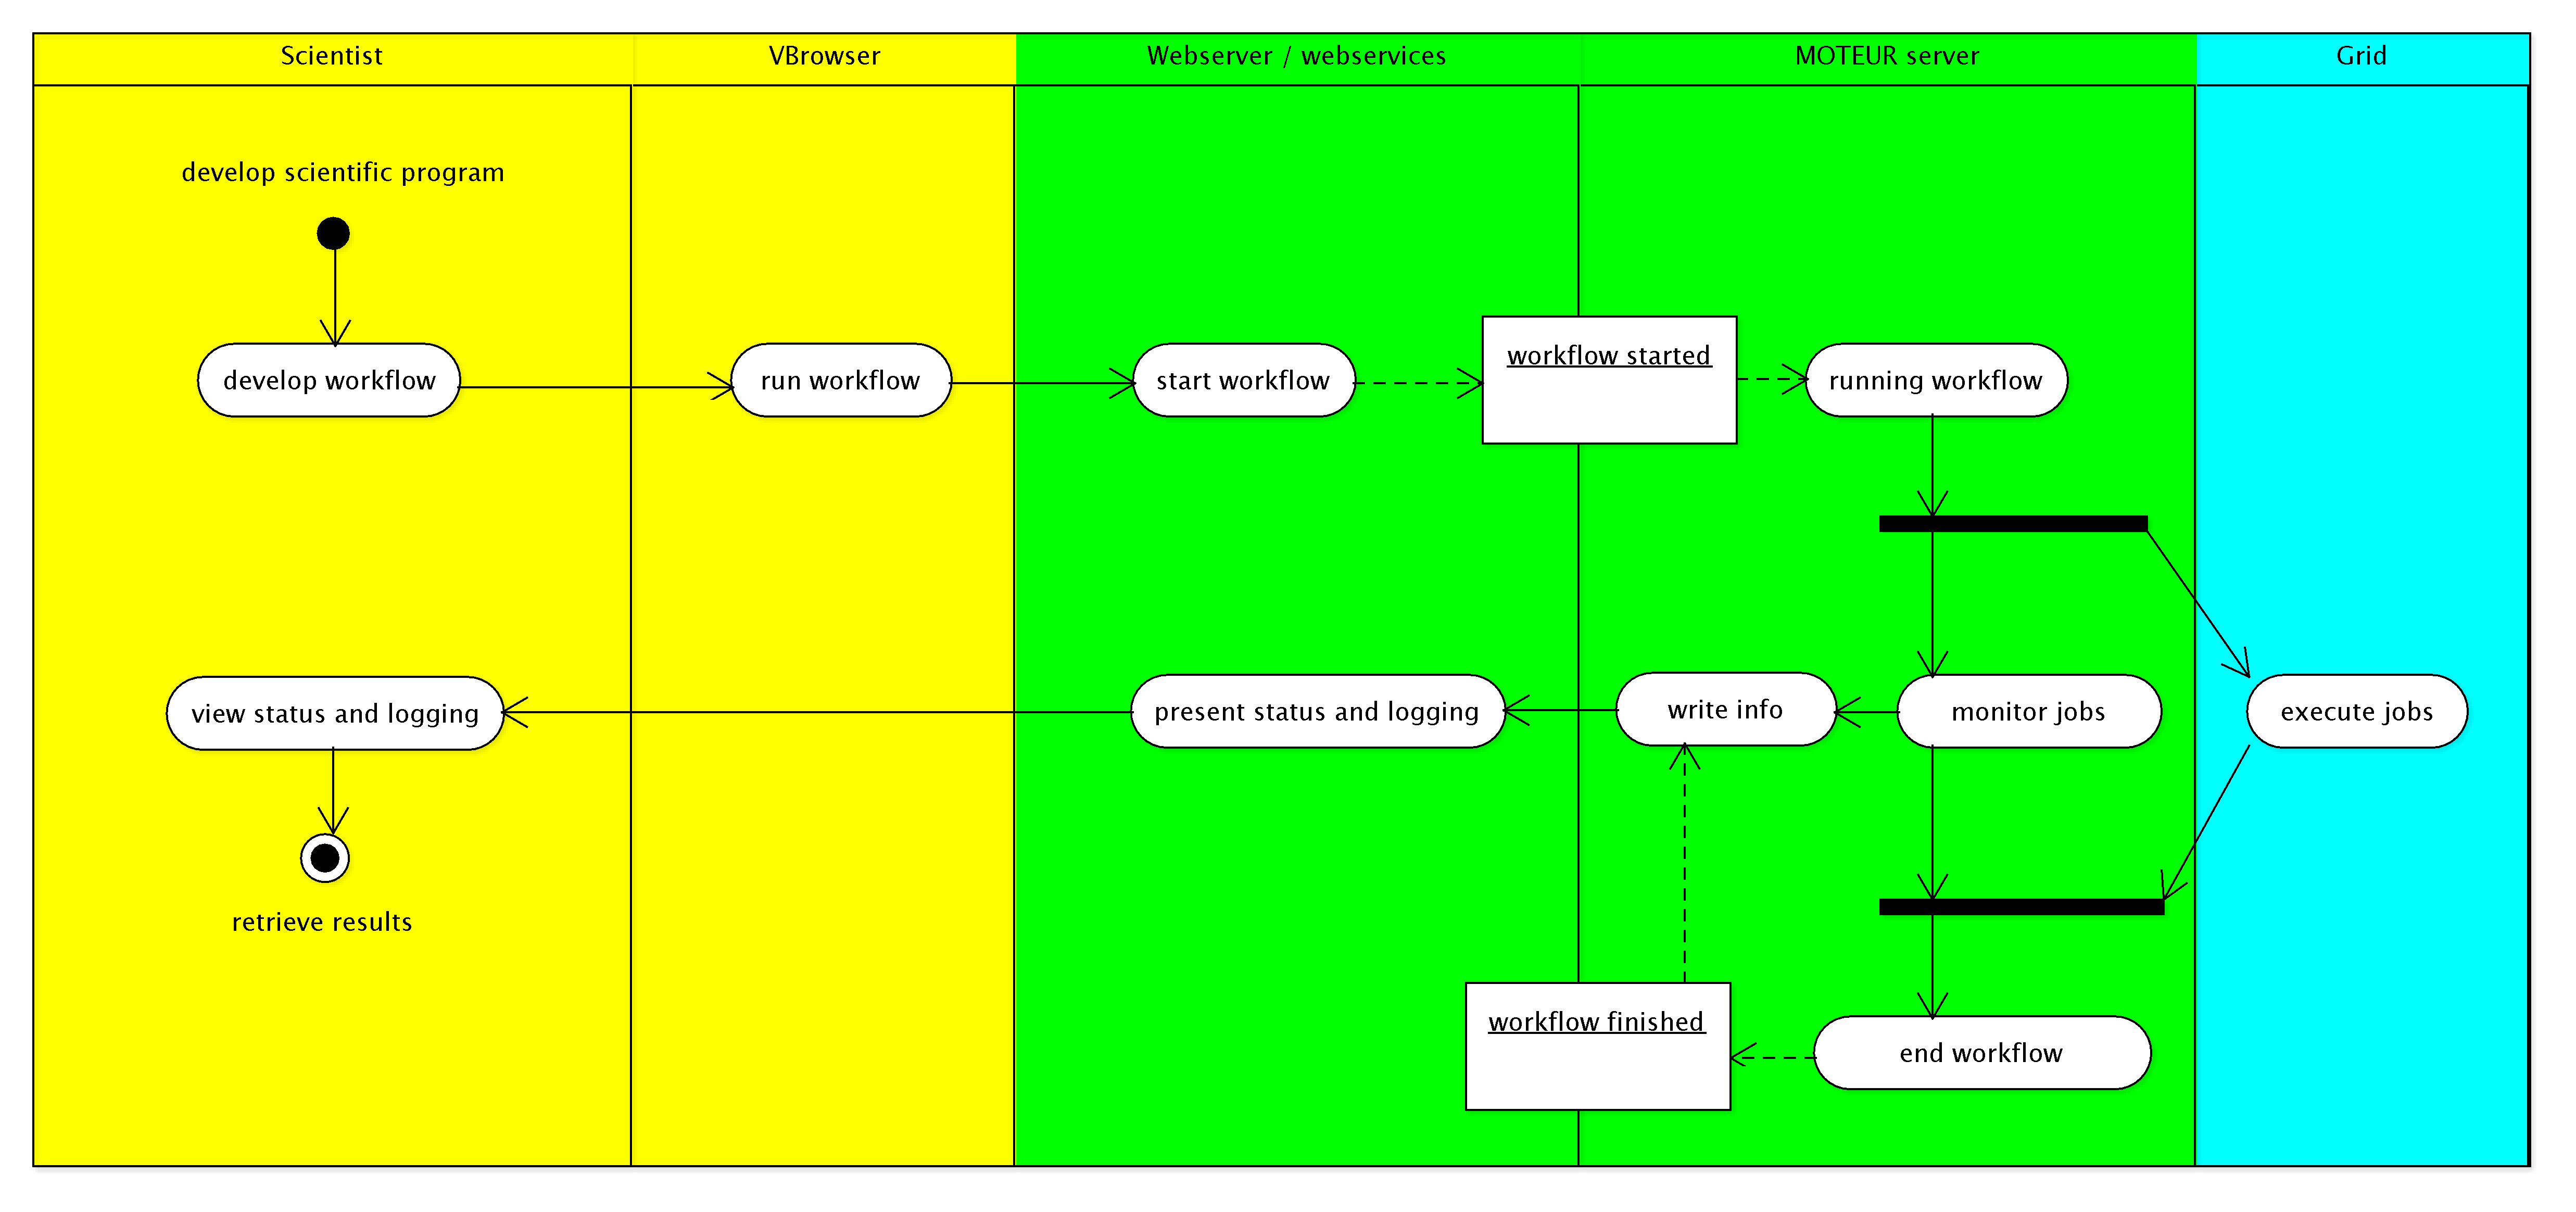
\includegraphics[width=7cm,height=3.5cm]{AMCgridresearch.png} 
  \caption{Diagram showing the applications involved in grid research in various domains. }
  \label{fig:gridapplications}
  \vspace{-0.5cm}
\end{figure}

\subsection{Problem description}
\noindent
The problem domain we focus on in this project is user feedback and support. To give you an idea of this problem domain we describe everyday life of a grid researcher:
\begin{itemize}
\item Developer implements application, develops a workflow that uses this application
\item Researcher starts the workflow from the VBrowser client
\item The workflow is executed on the grid by MOTEUR
\item Things are ok if all workflow tasks are executed successfully (even if after some retries)
\item If an error occurs, the researcher does not know what to do. The errors are associated to low level grid jobs, and not to workflow tasks (as the researcher knows them)
\item He/she contacts the developer, who dives (manually) into the logs at the various components and domains and  in turn contacts other specialists involved. 
\end{itemize}



\subsection{Solution}
\noindent
Thinking about ways to improve this situation we were looking for an approach that can deal with the cross domain and dynamic nature of the environment, that is non invasive, that can communicate about local issues with other parts of the environment, that can be extended with learning capabilities and with a common vocabulary. Agent technology, implemented in the FIPA compliant platform Jade, offers all this. We envisioned an agent based solution to provide support for the grid researcher and limit his or her tasks.

\begin{figure}[H]
  \vspace{-0.2cm}
  \centering
  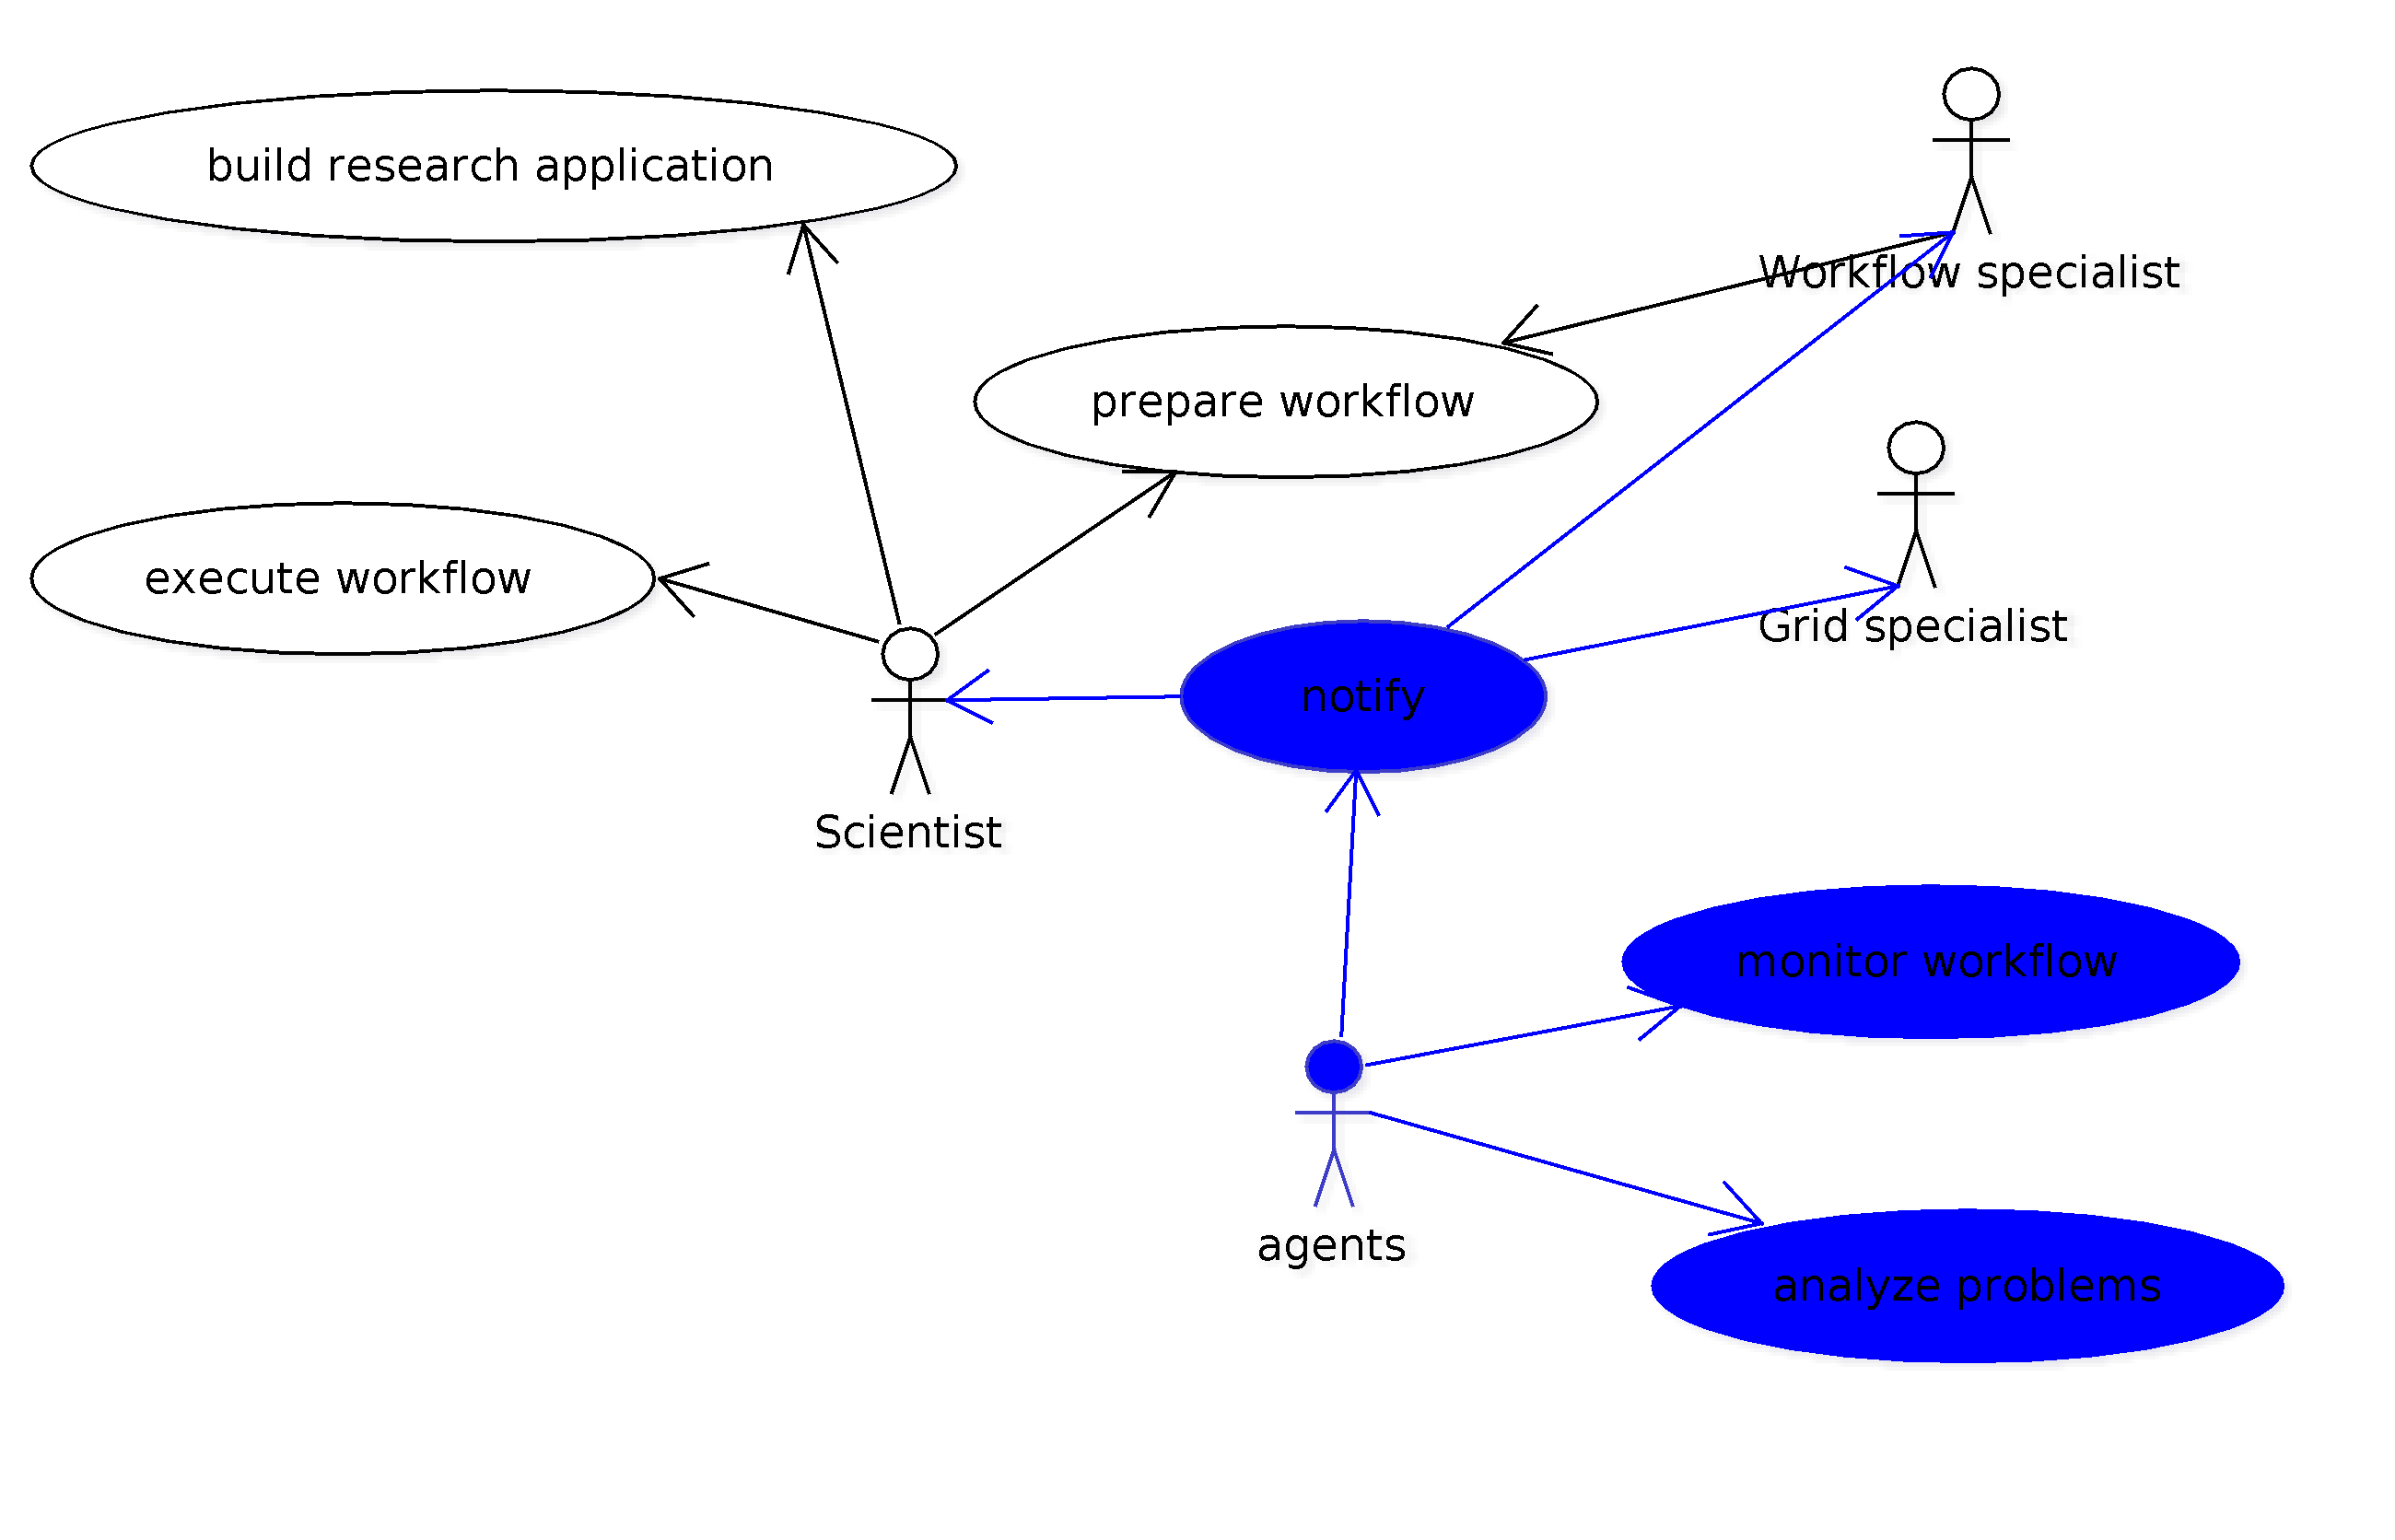
\includegraphics[width=7cm,height=5cm]{futureusecasegridresearchamc.png} 
  \caption{Usecase diagram showing tasks (in blue) that can be supported by agents. }
  \label{fig:futureusecase}
  \vspace{-0.5cm}
\end{figure}

We designed and implemented a non invasive agent layer in the chain of applications that is able to improve user support.

\begin{figure}[H]
  \vspace{-0.2cm}
  \centering
  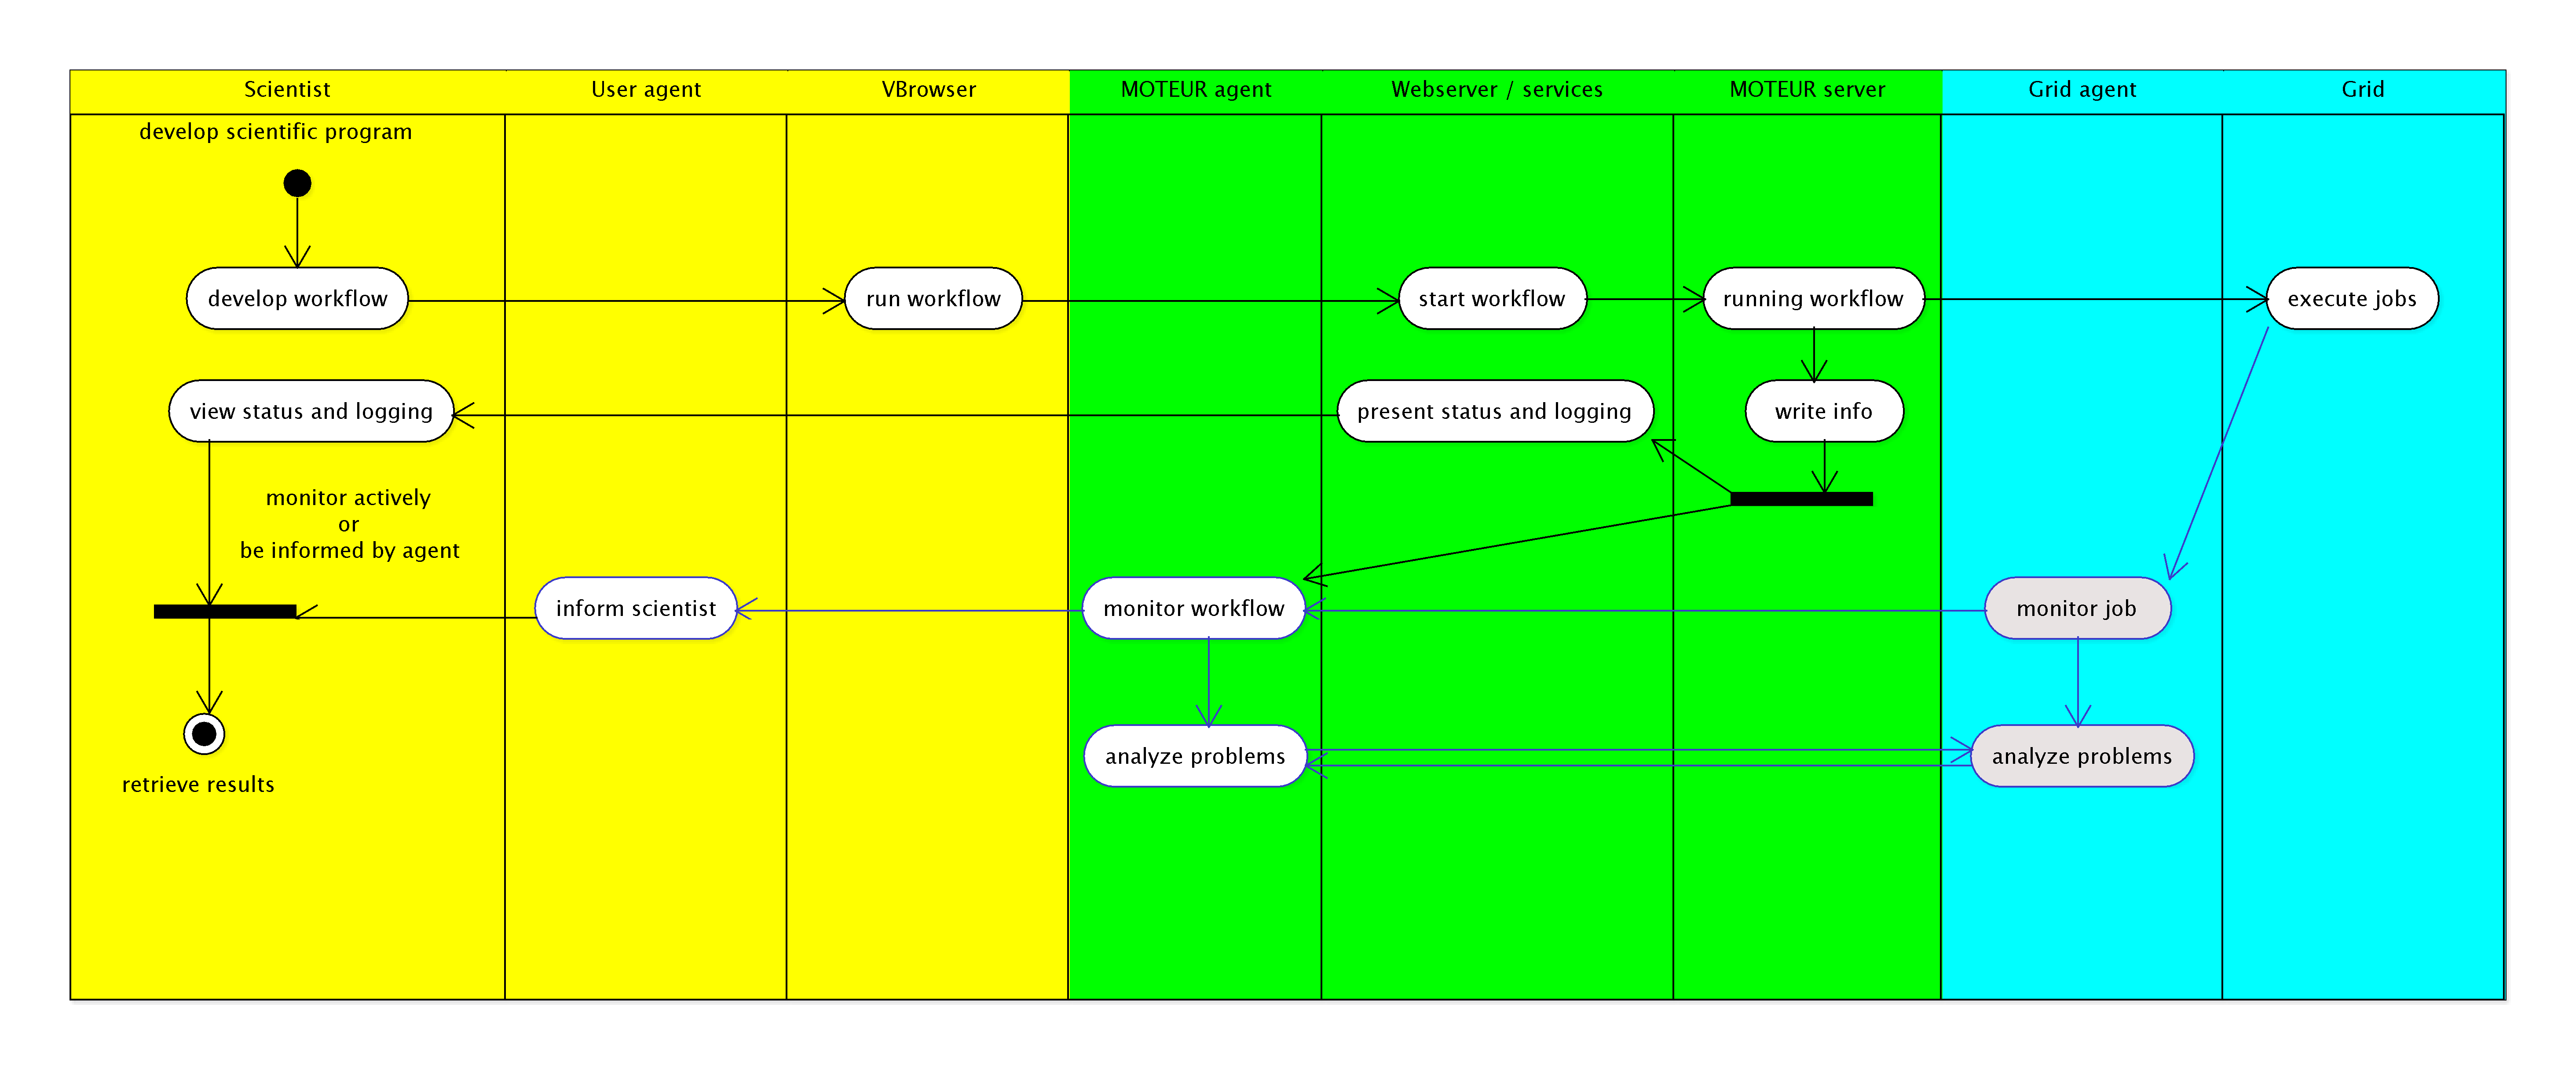
\includegraphics[width=7cm,height=3.5cm]{AMCgridresearchsupportedbyagents.png} 
  \caption{Diagram showing the agent support layer. }
  \label{fig:agentsupport}
  \vspace{-0.5cm}
\end{figure}

\pagebreak

Each individual workflow is supported by a group of agents, one to inform the user, one to monitor the progress of workflows and grid jobs and one to provide direct feedback from within the grid.

\begin{figure}[H]
  \vspace{-0.2cm}
  \centering
  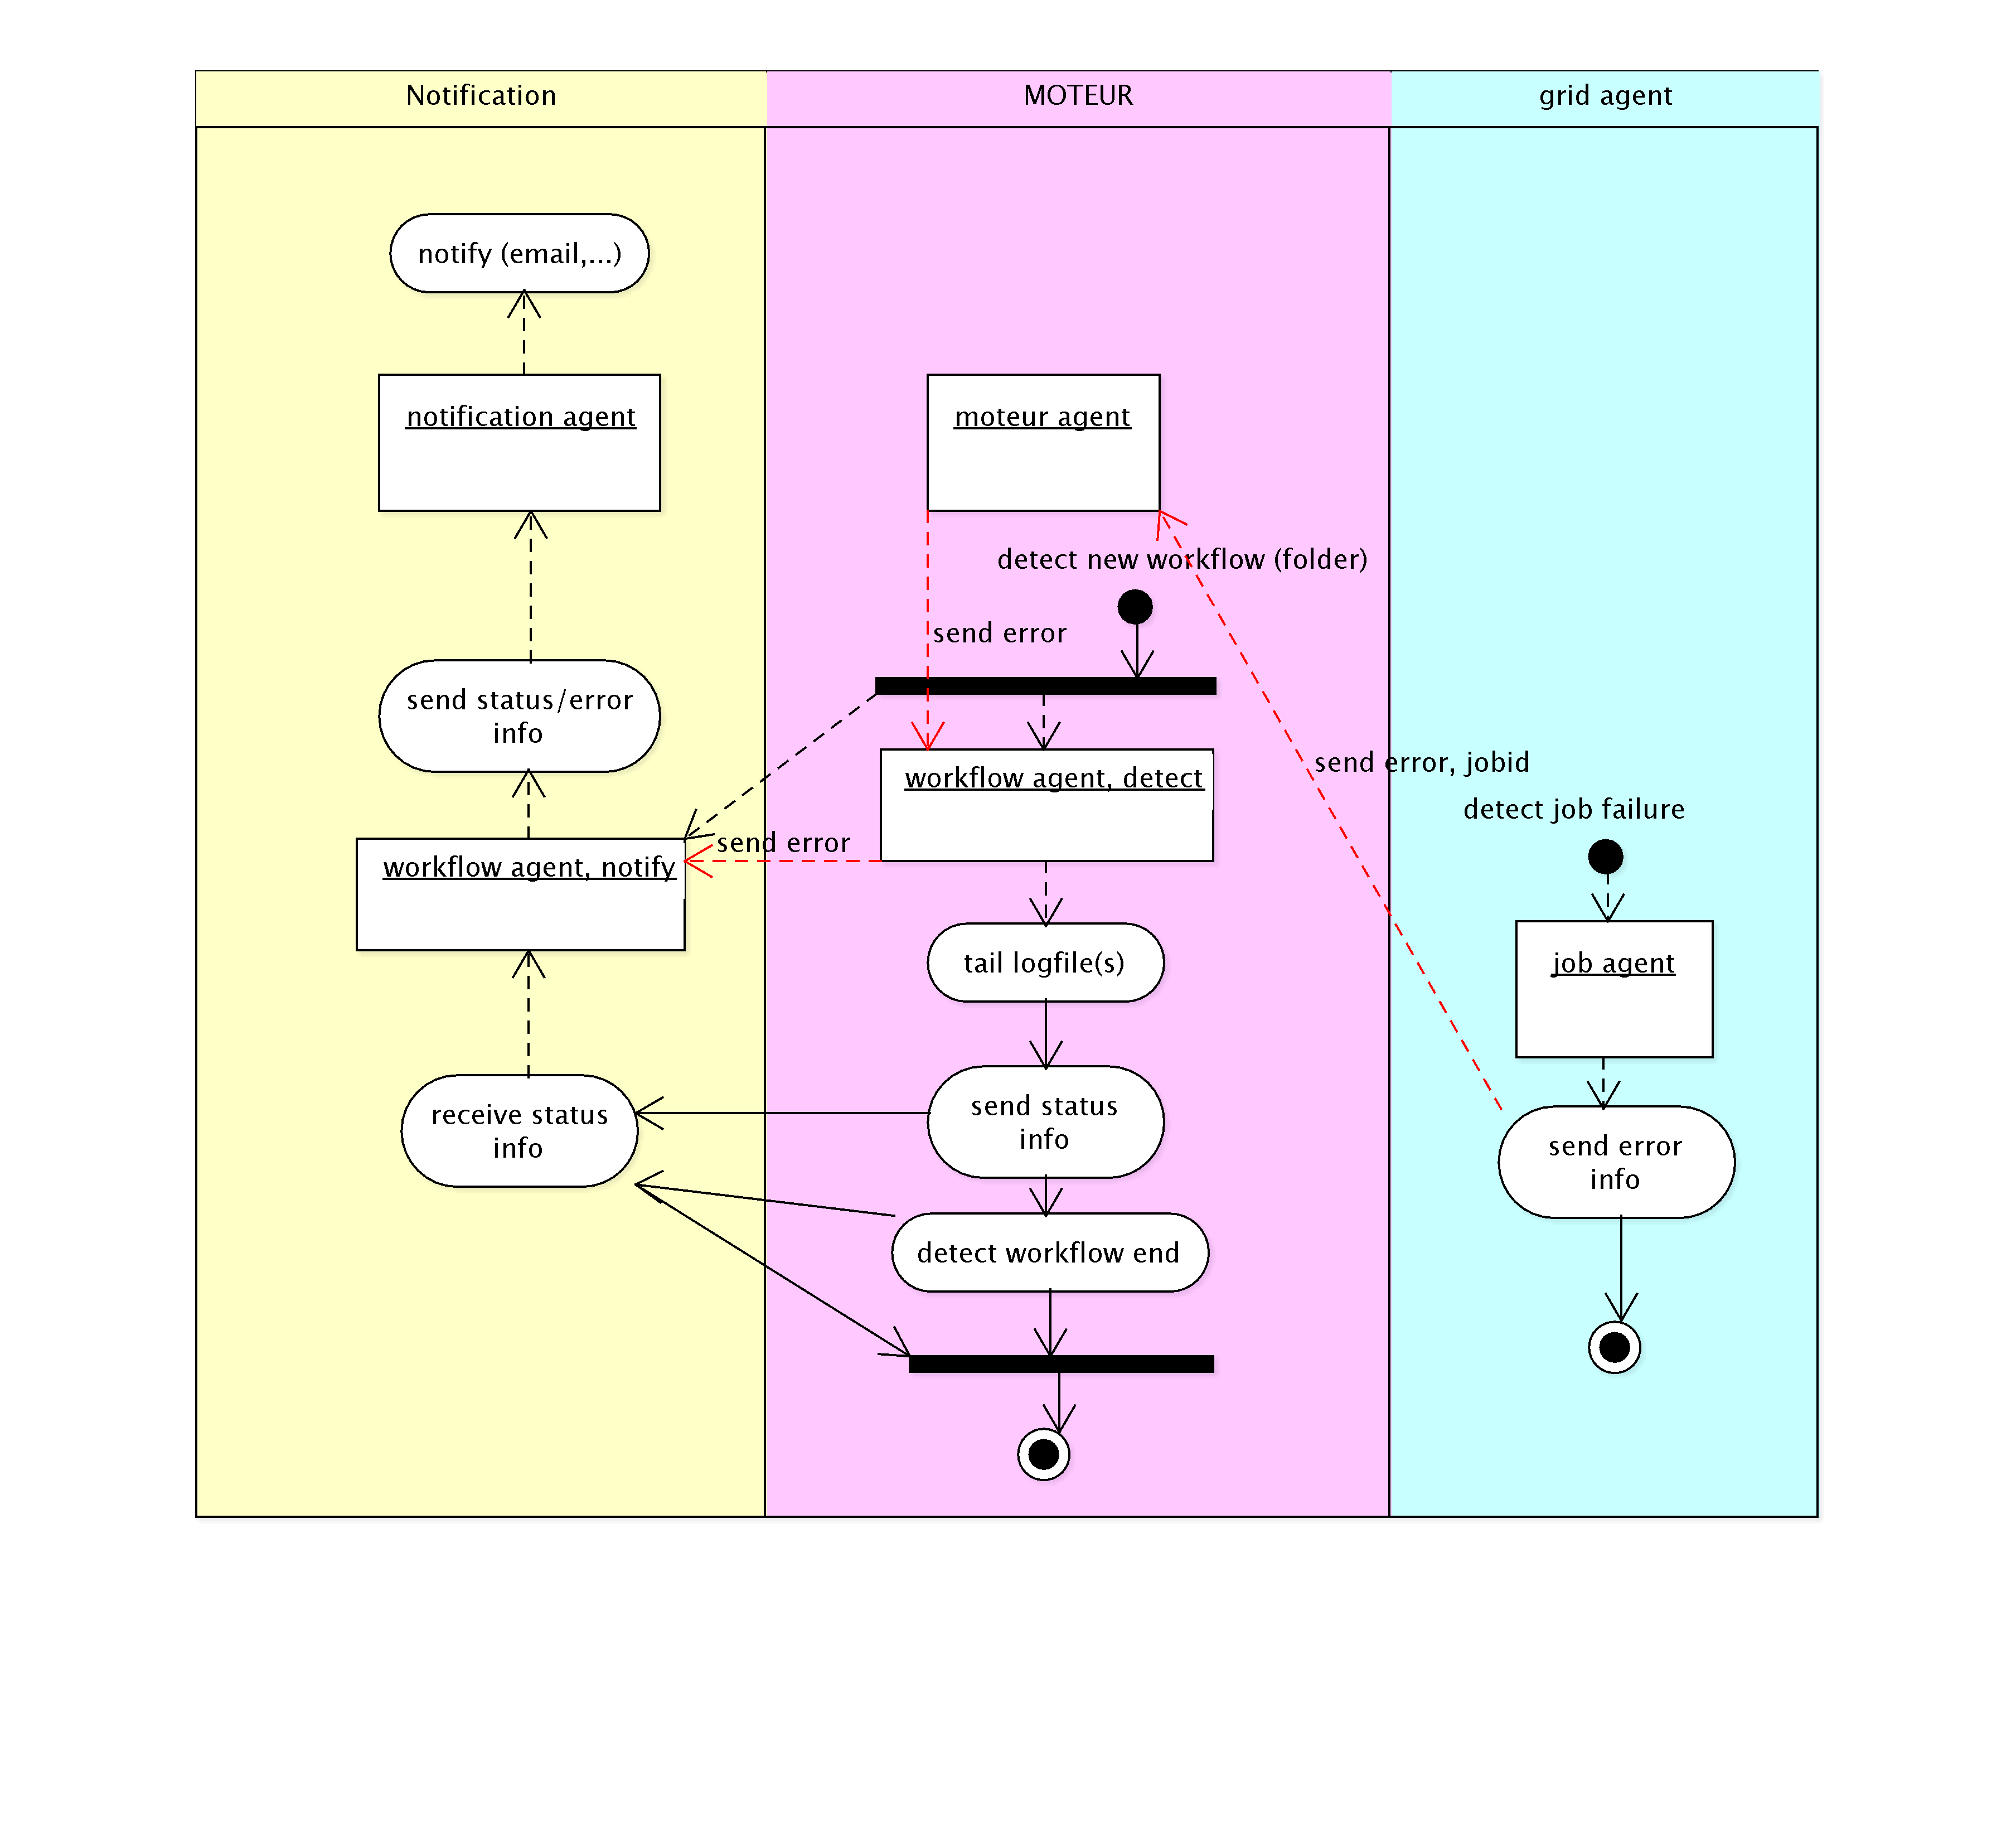
\includegraphics[width=8cm,height=8cm]{monitorworkflows.png} 
  \caption{Support agents for a workflow. }
  \label{fig:supportagents}
  \vspace{-0.5cm}
\end{figure}

\section{\uppercase{Results}}
\label{sec:results}
\noindent Quantified results have yet to be collected. Testing, also in a production environment, shows the solution is truly non invasive, flexible and very suitable in the cross domain environment. Especially feedback from grid jobs, as also shown in DIANE, is a powerful technique. Sometimes MOTEUR looses track of grid jobs or gets information on a job really slow, by arranging callback from within a grid job information can reach the researcher faster, sometimes upto half an hour.

\section{\uppercase{Conclusion}}
\label{sec:conclusion}
\noindent Non invasive user support by means of Agent Technology in grid research looks very promising and should be investigated and elaborated further. Initiatives envisioning similar techniques should join efforts and strive for standardization where this is desirable.
\subsection{(near) Future}
\noindent
The DUST project will continue at the AMC with a focus on some of the following ideas.
\begin{itemize}
\item prepare for evaluation of this concept by smart definition of goals, expectations, etc.
\item automate conversations using FIPA interaction protocols to speed up troubleshooting of problems
\item integrate 'callback on failure' for jobs at MOTEUR (workflow server)
\item introduce useful, user friendly 'personal agents' for people involved in the chain
\item support for dynamic configuration
\item introduce a Management GUI for the solution
\item build in support for a container per workflow (dynamic ports) to further improve security
\item semantic technologies? For what?
\end{itemize}



\section*{\uppercase{Acknowledgements}}
We would like to thank various people at the NIKHEF, CREATIS, Logica and the AMC, especially Silvia D. Olabarriaga, who made this project possible.

\end{document}
